\documentclass[12pt]{article}

\usepackage{titlesec}
\usepackage{enumerate}
\usepackage[parfill]{parskip}
\usepackage{amsmath}
\usepackage{amssymb}
\usepackage{amsthm}
\usepackage{caption}
\usepackage{subcaption}
\usepackage{float}
\usepackage{graphicx}
\usepackage{verbatim}
\usepackage{listings}
\usepackage{cleveref}

\usepackage{xcolor}

\definecolor{codegreen}{rgb}{0,0.6,0}
\definecolor{codegray}{rgb}{0.5,0.5,0.5}
\definecolor{codepurple}{rgb}{0.58,0,0.82}
\definecolor{backcolour}{rgb}{0.95,0.95,0.92}

\lstdefinestyle{mystyle}{
    language=Python,
    backgroundcolor=\color{backcolour},   
    commentstyle=\color{codegray},
    keywordstyle=\color{codegreen},
    numberstyle=\tiny\color{codegray},
    stringstyle=\color{codepurple},
    basicstyle=\ttfamily\scriptsize,
    breakatwhitespace=false,         
    captionpos=b,                    
    keepspaces=true,                 
    numbers=left,                    
    numbersep=5pt,                  
    showspaces=false,                
    showstringspaces=false,
    showtabs=false,                  
    tabsize=2
}

\lstset{style=mystyle}

\makeatletter
\newcommand{\verbatimfont}[1]{\def\verbatim@font{#1}}%
\makeatother

\titleformat{\section}
    {\normalfont\fontsize{15}{17}\bfseries}{\thesection}{2.27em}{}
\titleformat{\subsection}
    {\normalfont\fontsize{17}{18}\bfseries}{\thesubsection}{1em}{}
\titleformat{\subsubsection}
    {\normalfont\fontsize{15}{15}\bfseries}{\arabic{subsubsection}}{1em}{}

\newcommand{\starreditem}{\item[\refstepcounter{enumi}\number\value{enumi}*.]}

\newtheorem*{prop}{Proposition}

\begin{document}
\setcounter{section}{16}
\section{Combinatorics}
\setcounter{subsection}{6}
\subsection{Graph planarity}
\emph{CATAM coursework for Part II of the Mathematical Tripos. Sections have
been numbered as they appear in the manual.}

\subsubsection{Graph drawing}
\textbf{Question 1}\quad 
Given a graph \(G\) with a cycle \(C\) containing vertices \(v_1,v_2,...,v_m\)
(in order), we assign to each \(v_i\) the coordinates \((\sin \frac{2\pi i}{m},
\cos\frac{2\pi i}{m})\) so that the cycle occupies a regular \(m\)-gon. Let
\(V[G]\setminus\{v_1,...,v_m\}=\{w_1,...,w_n\}\) be the vertices not in the
cycle, and  write \((x_i,y_i)\) for the coordinates of \(w_i\). Define two
matrices to record adjacency
\[\Delta_{ij} = \begin{cases} 1, &\text{ if }\{w_i,w_j\}\in E[G] \\ 0, &\text{
    if }\{w_i,w_j\}\notin E[G] \end{cases}, \qquad \Omega_{ij} = \begin{cases} 1, &\text{ if }\{w_i,v_j\}\in E[G] \\ 0, &\text{ if }\{w_i,v_j\}\notin E[G] \end{cases}.\]
If \(C\) has a single bridge, Tutte's theorem provides a way to calculate the
coordinates \((x_i,y_i)\) such that the representation of \(G\) is planar: 
\begin{gather*}
    x_i = \frac{\sum_{j=1}^n \Delta_{ij}x_j + \sum_{j=1}^m
\Omega_{ij}\sin \frac{2\pi j}{m} }{d(w_i)}, \quad 
    y_i = \frac{\sum_{j=1}^n \Delta_{ij}y_j + \sum_{j=1}^m
\Omega_{ij}\cos \frac{2\pi j}{m} }{d(w_i)}.
\end{gather*}
Defining three new matrices by 
\begin{gather*}
    A_{ij}=\begin{cases}-\Delta_{ij}, &i\neq j\\ 
    d(w_i), &i=j\end{cases}, \quad
    S_i = \sum_{j=1}^m \Omega_{ij}\sin\frac{2\pi j}{m}, \quad
    T_i = \sum_{j=1}^m \Omega_{ij}\cos\frac{2\pi j}{m}, \quad
\end{gather*}
we can express Tutte's formula for the coordinates succintly as 
\[A\begin{pmatrix} x_1 \\ \vdots \\ x_n\end{pmatrix} = S, \quad 
  A\begin{pmatrix} y_1 \\ \vdots \\ y_n\end{pmatrix} = T. \]
  The coordinates of the vertices can now be obtained by calculating \(A^{-1}S\)
  and \(A^{-1}T\). Using the above method, we produce planar representations of the five
  platonic solids and the graph \(K2+P5\):

  \begin{figure}[H]
      \centering 
      \begin{subfigure}[b]{0.3\textwidth}
          \centering 
          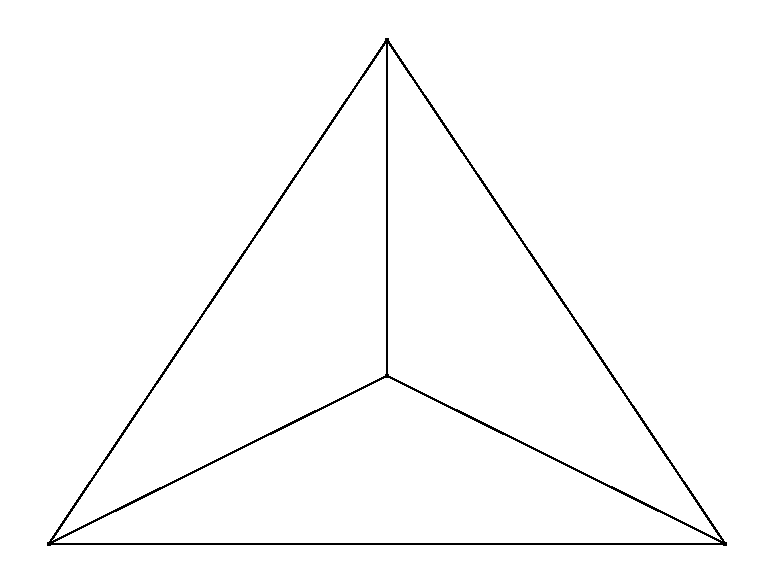
\includegraphics[width = \textwidth]{../output/Q1-platonic-4.pdf}
          \caption{The tetrahedron}
      \end{subfigure}
      \hfill
      \begin{subfigure}[b]{0.3\textwidth}
          \centering 
          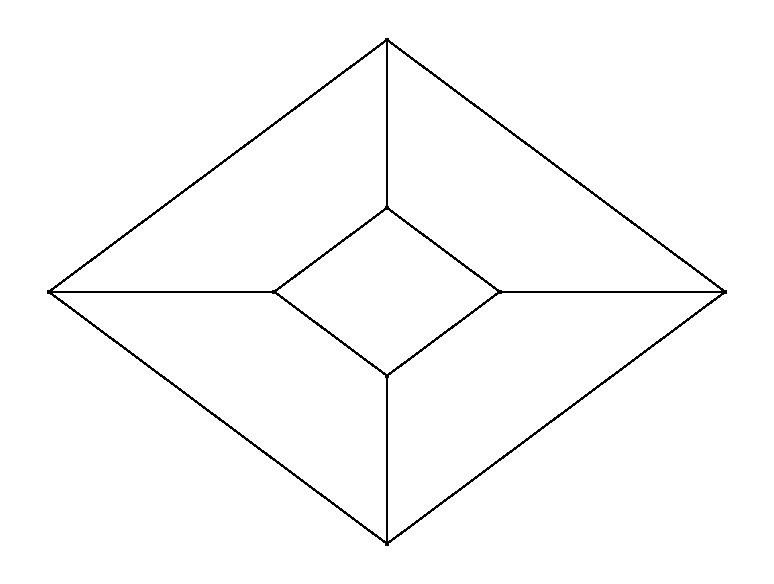
\includegraphics[width = \textwidth]{../output/Q1-platonic-6.pdf}
          \caption{The cube}
      \end{subfigure}
      \hfill
      \begin{subfigure}[b]{0.3\textwidth}
          \centering 
          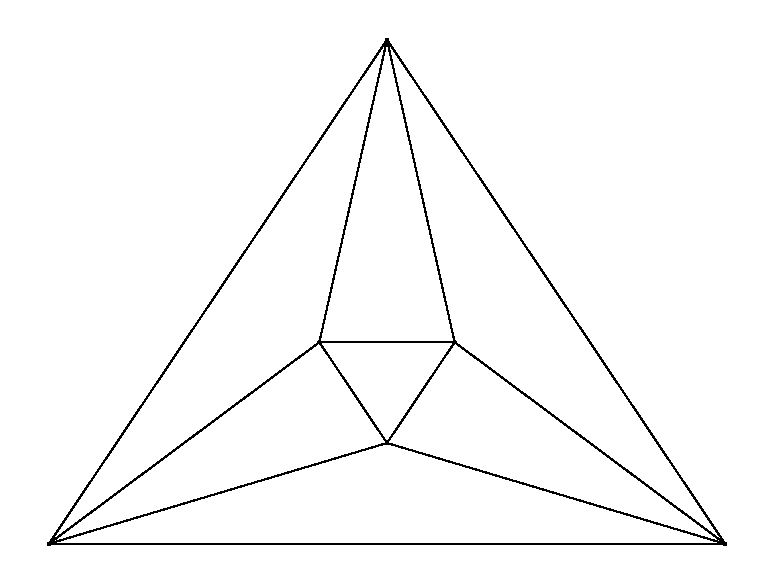
\includegraphics[width = \textwidth]{../output/Q1-platonic-8.pdf}
          \caption{The octahedron}
      \end{subfigure}
      \hfill
      \begin{subfigure}[b]{0.3\textwidth}
          \centering 
          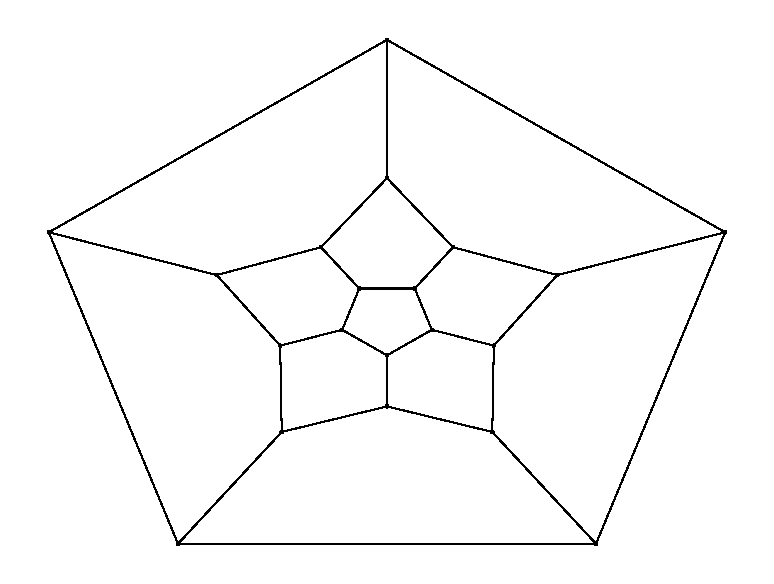
\includegraphics[width = \textwidth]{../output/Q1-platonic-12.pdf}
          \caption{The icosahedron}
      \end{subfigure}
      \hfill
      \begin{subfigure}[b]{0.3\textwidth}
          \centering 
          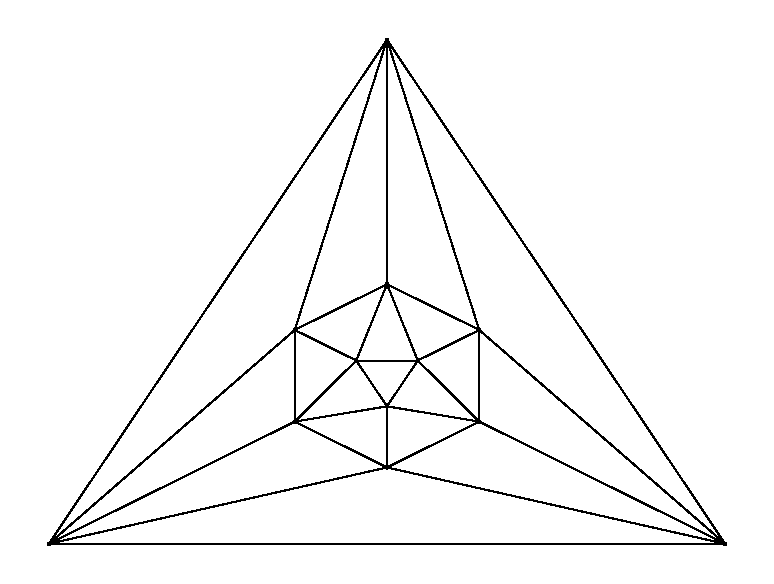
\includegraphics[width = \textwidth]{../output/Q1-platonic-20.pdf}
          \caption{The dodecahedron}
      \end{subfigure}
      \hfill
      \begin{subfigure}[b]{0.3\textwidth}
          \centering 
          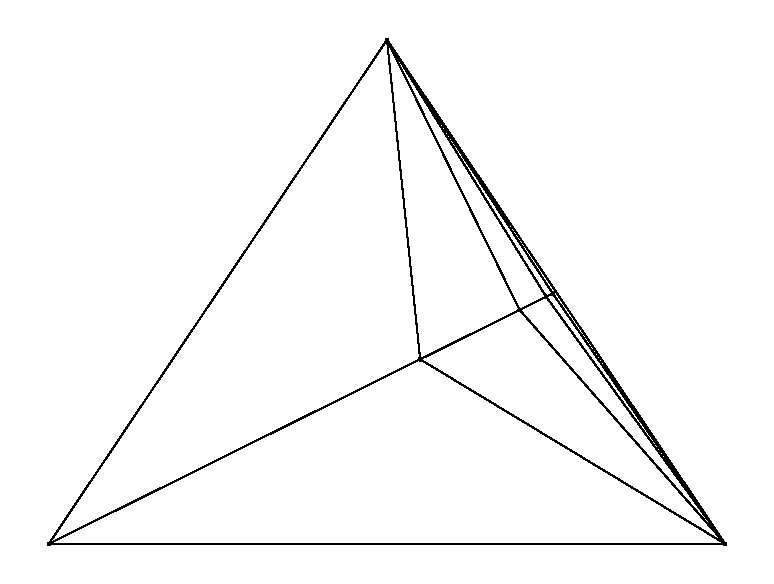
\includegraphics[width = \textwidth]{../output/Q1-k2-plus-p5.pdf}
          \caption{\(K2+P5\)}
      \end{subfigure}
      \hfill
      \caption{Six planar graphs plotted using Tutte's method.}
  \end{figure}
  While Tutte's formula works very well for graphs possessing a high number of
  symmetries, the disadvantage is apparent for graphs like \(K2+P5\) where the
  vertices are skewed in a particular direction leading to sub-optimal
  representations. If we understand the graph sufficiently well, this can be
  counteracted by applying appropriate weights to the vertices.

\subsubsection{Bridges and components}
\textbf{Question 2}\quad 
For a set \(U\subset V[G]\), define the \emph{neighbourhood} of \(U\) by  \(\Gamma(U)=\bigcup_{x\in U}\Gamma(x) \cup U\). Write \(\Gamma^n(U)=\Gamma(\Gamma^{n-1}(U))\), where \(\Gamma^0(U)=U\). For any vertex \(v\in V[G]\), the sequence \(\{v\},
\Gamma\{v\}, \Gamma^2\{v\},...\) is \(\subset\)-increasing and bounded
above by \(V[G]\), hence stabilises in finitely many steps and the fixed point
is a connected component of \(G\) containing \(v\). Repeating this
process, we can find all the connected components of the graph.

Finding the bridges of a cycle \(C\) now is straightforward by finding the connected
components of \(G\setminus V[C]\), and the vertices of attachment can be found
by examining the edges connecting \(C\) to these components. Chords need to be
found separately by examining the vertices in the cycle pairwise.

\subsubsection{Interleaving}
\textbf{Question 3}\quad Suppose \(G\) is a planar graph, then every subgraph of
\(G\) is planar. If \(C\) is a cycle in \(G\) with \(\ell\) bridges
\(B_1,...,B_\ell\), choose a planar representation of \(G\). In this
representation, the cycle \(C\) is a simple closed curve, hence\footnote{by the Jordan
curve theorem} splits the plane into two regions-- call them the \emph{inside}
and the \emph{outside}. Since a bridge is connected, it must entirely lie in the
(topological) closure of one of these regions. Now a bridge contains
a path between its vertices of attachment which does not intersect the cycle
except at its end points. Moreover, distinct bridges can only meet at their
vertices of attachment. If \(a,b,c,d\) are distinct vertices
appearing on the cycle in that order such that \(a,c\) are vertices of attachment
of the bridge \(B_i\) and \(b,d\) are vertices of attachment of the bridge \(B_j
\) (not equal to \(B_i\)), then \(B_i\) contains an \(a-c\) path while \(B_j\)
contains a \(b-d\) path; and the only way these paths don't intersect is if they
lie in different regions. It follows that \(B_i\) and \(B_j\) must themselves lie in different regions. On the other hand, suppose the vertices of attachment of both \(B_i\) and \(B_j\) are
precisely \(a,b,c\) (all distinct). In particular, neither of the bridges is a
chord so we can pick a vertex \(x\in V[B_i]\setminus V[C]\). Without loss of
generality \(B_i\) is drawn on the inside of the plane, so that the
\(x-a,x-b,x-c\) paths contained in \(B_i\) (along with the cycle \(C\)) divide
the plane into four disjoint regions (the outside, and the three subdivisions of
the inside). The drawing of \(B_j\) must lie in one of the regions, and moreover
that region must have all three of the vertices of attachment on its boundary.
The only such region is the outside. We have thus shown that any two
interleaving graphs lie in different regions of the plane-- this induces a
bipartition of the interleave graph \(H\) of \(G\).

Conversely, suppose each of the subgraphs \(G_i\) with edges \(E(C)\cup B_i\)
(\(1\leq i \leq \ell\)) is planar and the interleave graph \(H\) is bipartite.
Choose a bipartition \(V[H]=A\cup B\) of \(H\). Since \(G_i\) is a cycle with a single bridge,
Tutte's theorem allows for a planar drawing where \(C\) occupies a regular
polygon and every other vertex of \(B_i\) is placed in the centroid of its
neighbours. In particular, the entire drawing of \(B_i\) lies in the convex
polygon determined by its vertices of attachment. If \(i,j\in A\) (likewise
\(B\)) are distinct, the bridges \(B_i\) and \(B_j\) do not
interleave, and hence the convex hulls of their vertices of attachments are
disjoint. It follows that the subgraph \(G_A\) with edges \(E(C)\cup \bigcup_{i\in
A}B_i\) is planar, and has a drawing where \(C\) occupies a regular polygon and
every other vertex is at the centroid of its neighbours. A similar drawing is
produced for \(G_B\), the subgraph with edges \(E(C)\cup \bigcup_{i\in B}B_i\).
Now observing that planar graphs are in fact graphs on a sphere (by considering
steriographic projection, for instance), we produce spherical drawings of
\(G_A\) and \(G_B\) such that \(C\) occupies the equator. These drawings can be
put together such that \(G_A\) and \(G_B\) lie in opposite hemispheres (and they
agree on \(C\))-- resuting in a spherical drawing of \(G\). By projecting
steriographically on the plane, conclude that \(G\) is planar.

\subsubsection{The core of a graph}
\textbf{Question 6}\quad 
Suppose \(G\) is a graph of minimum degree at least two. Then pick a vertex
\(x_1\)-- this has two distinct neighbours \(x_0\) and \(x_2\), giving a path
\(x_0x_1x_2\) in \(G\). Having constructed a path \(x_0x_1...x_n\) (all vertices
distinct, \(n\geq 2\)), observe that \(x_n\) has a neighbour \(y\neq
x_{n-1}\). If \(y\in \{x_0,...,x_{n-2}\}\)-- say \(y=x_i\), we have found a
cycle \(x_ix_{i+1}...x_n\) in \(G\). Otherwise, we have a longer path
\(x_0x_1...x_{n}y\) and can repeat the procedure. But the graph is finite, hence
the process terminates and we find a cycle in finite time. 

Likewise, suppose \(G\) has minimum degree at least three. From above, we have a
path \(x_0x_1x_2\). In fact, \(x_2\) must have a neighbour \(x_3\neq x_0,x_1\),
giving a path \(x_0x_1x_2x_3\). Having constructed a path \(x_0x_1...x_n\)
(\(n\geq 3\)), observe that \(x_n\) has two distinct neighbours \(y,z\), neither
equal to \(x_{n-1}\). If both lie in \(\{x_0,...,x_{n-2}\}\)-- say \(y=x_i\),
\(z=x_j\) for \(i<j\), we have found a cycle \(x_ix_{i+1}...x_{n}\) in \(G\) and
this has a chord \(x_nx_j\). Otherwise, we have found a longer path
\(x_0x_1...x_ny\), and can repeat the procedure. This algorithm is again
guaranteed to terminate by the finiteness of \(G\).

\subsubsection{A planarity algorithm}
\textbf{Question 7}\quad 
Since the operations involved in finding the core decrease the number of
vertices, the process terminates and we can find the core \(G^\ast\) of \(G\) in
finite time. It is clear that a graph is planar if and only if its core is; in
particular, if \(G^\ast\) is empty then \(G\) is planar. If \(G^\ast\) is
non-empty, it has minimum degree \(3\) hence contains a cycle \(C\) with a chord
\(e\). We have already exhibited terminating algorithms for finding such a
cycle with a chord, and constructing its interleave graph \(H\). Suppose the
bridges of \(C\) are \(B_1,...,B_\ell\) where \(B_1=\{e\}\). Note that the
subgraph with edges \(E(C)\cup B_1\) is planar since it is a cycle with a chord.
From the discussion in Queston 3, if \(H\) is not bipartite then \(G\) is not
planar-- and we have a terminating algorithm to check if a graph is bipartite (in fact,
to produce a bipartition). If \(H\) is bipartite, then \(G^\ast\) is planar if and
only if each of the subgraphs with edges \(E(C)\cup B_i\) (\(2\leq i \leq
\ell\)) is planar. Lastly, observe that \(C\) is a  cycle in \(G^\ast - e\) with
bridges \(B_2,...,B_\ell\), and the corresponding interleave graph is a subgraph
of \(H\). Thus \(H\) (and hence its subgraphs) being bipartite, \(G^\ast\) is
planar if and only if \(G^\ast - e\) is.
Since at each step of the recursion we either terminate by deciding the
planarity of \(G\) or reduce the problem to checking the planarity of a graph with strictly
fewer edges, the algorithm must terminate.

\textbf{Question 8}\quad 
We implement the above algorithm and test it on the following graphs: 
\begin{enumerate}[(i)]
    \item \(K2+P5\), which we know is planar.
    \item \(K3,3\), which from Kuratowski's theorem is non-planar.
    \item \(K5\), which from Kuratowski's theorem is non-planar.
    \item The dodecahedron \(P_{12}\), which we know is planar.
    \item \(P_{12}\) with two edges added-- since the every face of the
        dodecahedron is a triangle, it is maximal planar hence adding any edges
        makes it non-planar.
\end{enumerate}
In each case, the algorithm returns the expected output.

\textbf{Question 9}\quad 
If \(G\) is a maximal planar graph on \(n\) vertices, observe that each face of
\(G\) must be a triangle-- else we could subdivide a non-triangular face to get
a planar graph which has \(G\) as a proper subgraph. Then each face is
surrounded by three edges and each edge by two faces, so if a planar
representation of \(G\) has \(F\) faces and \(E\) edges, we can write  
\[\#\{(f,e)\;|\;f\text{ a face, } e\text{ an edge surrounding }f\} = 3F = 2E.\]
Combined with Euler's formula \(n-E+F=2\), we have \(E= 3n-6\). 

Starting with the empty graph on \(n\) vertices and adding each of the
\(\binom{n}{2}\) edges in random order as long as planarity is preserved, the
graph we end up with is indeed maximal planar, hence has \(3n-6\) edges. 

\begin{prop}
    Suppose \(G\) is a maximal planar graph on \(n\geq 4\) vertices. Then \(G\)
    is 3-connected and contains a cycle with exactly one bridge.
    \begin{proof}
        Let \(G\) be a maximal planar graph on \(n\geq 4\) vertices. Pick a
        planar representation of \(G\). Call an edge \(e\) \emph{contractible}
        if the only triangles containing \(e\) are faces (i.e.\ its end points
        have at most two common neighbours). Write \(G/e\) for
        the graph formed by contracting the edge \(e\), i.e.\ identifying its
        end points. This is still planar by Wagner's criterion since contracting
        an edge cannot create new minors.  Moreover, we lose exactly \(3\) edges
        in the contraction hence \(G/e\) contains \(n-1\) vertices and \(3n -
        9\) edges. It follows that \(G/e\) is maximal planar.

        We show by induction that \(G\) contains at least \(n\) contractible
        edges: clear if \(n=4\). If \(n>4\), take a planar representation of
        \(G\) and choose a triangle in \(G\) that is not a face. The subgraphs
        \(G_1\) and \(G_2\) contained (topologically) inside and outside the
        triangle are both maximal planar and together have \(|G_1|+|G_2| =
        n+3\) vertices, giving \(n+3\) possible candidates for contractible
        edges. Then in \(G\), all of these continue to remain contractible
        except for (possibly) the edges of the triangle, which can lose the
        property. Hence \(G\) contains at least \(n\) contractible edges.  

        Now suppose there are maximal planar graphs on \(4\) or more vertices
        which are not \(3\)-connected. Choose \(G\) to be such a graph with the
        minimal number of vertices, then there are \(u,v\in V(G)\) such that
        \(G-\{u,v\}\) is disconnected. Let the components be \(G_1\) and
        \(G_2\). Note that \(G\) has \(>4\) vertices since the only maximal
        planar graph on \(4\) vertices is \(K_4\). From the above discussion, we
        can pick an \(e\in E(G)\)
        which is contractible, then without loss of generality this edge must
        lie in \(G_1\). We observe that \(G/e\) is maximal planar with \(n-1\geq
        4\)
        vertices, and removing (the possibly modified versions of) \(\{u,v\}\)
        still disconnects \(G/e\). But \(G\) was chosen to be minimal, a
        contradiction. Hence every maximal planar graph on \(4\) or more
        vertices is \(3\)-connected.

        Choose a planar representation of \(G\) and let \(C\) be the \(3\)-cycle
        bounding a face. \(C\) has at least one bridge, and all the bridges lie
        in the (topological) complement of the face bounded by \(C\). If there
        were multiple such bridges, we could add edges connecting their bodies
        while preserving the planarity of \(G\); this contradicts the maximality
        of \(G\). Hence the boundary of a face in \(G\) has exactly one bridge.
    \end{proof}
\end{prop}

We generate twenty random maximal
planar graphs on \(40\) vertices. Now any edge \(x-y\) of such a graph bounds some face,
hence is a part of some \(3\)-cycle with exactly one bridge. We can iterate over
all the other vertices \(z\in V[G]\setminus \{x,y\}\) till we find such a cycle
\(xyz\), which we use as the outermost face in our plot. The proposition then
guarantees that Tutte's plotting algorithm works, so we use it to exhibit
planar representations of a selection of the graphs generated in
\cref{randomplots}. Appendix A contains edge-lists for the graphs shown.

  \begin{figure}[H]
      \centering 
      \begin{subfigure}[b]{0.45\textwidth}
          \centering 
          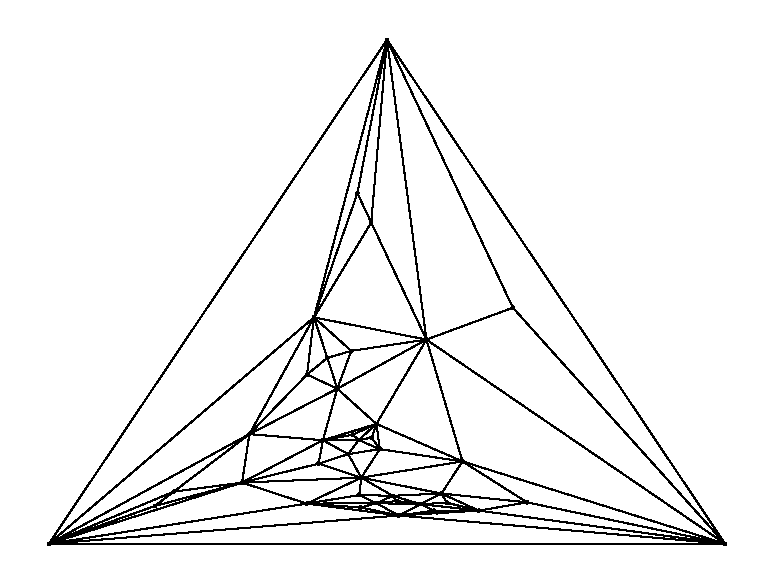
\includegraphics[width = \textwidth]{../output/Q9-random-405.pdf}
          \caption{Graph number 1}
      \end{subfigure}
      \hfill
      \begin{subfigure}[b]{0.45\textwidth}
          \centering 
          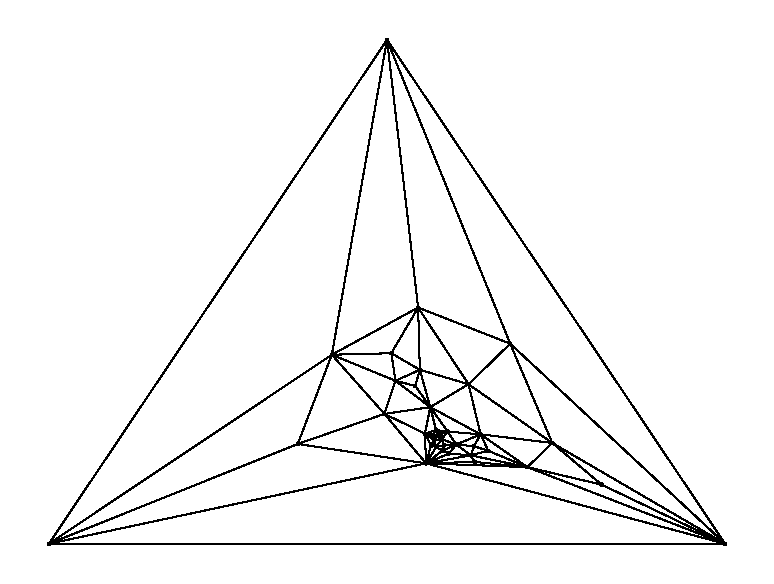
\includegraphics[width = \textwidth]{../output/Q9-random-409.pdf}
          \caption{Graph number 2}
      \end{subfigure}
      \hfill
      \begin{subfigure}[b]{0.45\textwidth}
          \centering 
          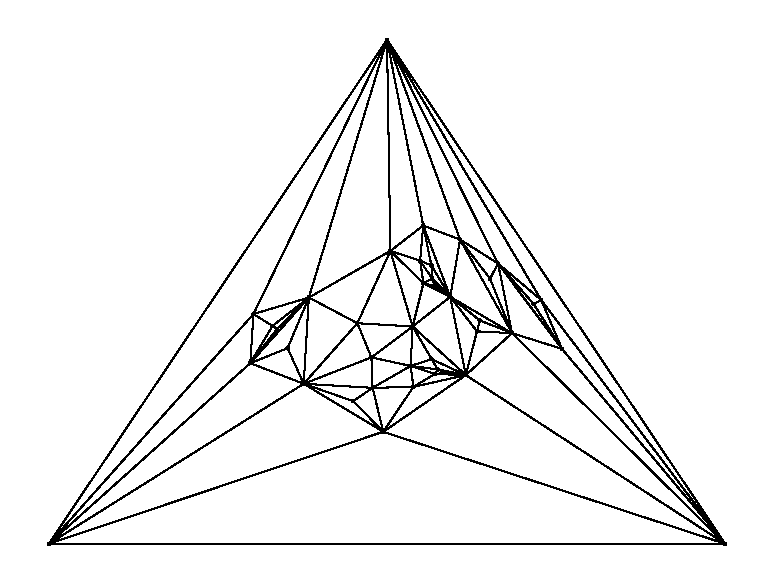
\includegraphics[width = \textwidth]{../output/Q9-random-4012.pdf}
          \caption{Graph number 3}
      \end{subfigure}
      \hfill
      \begin{subfigure}[b]{0.45\textwidth}
          \centering 
          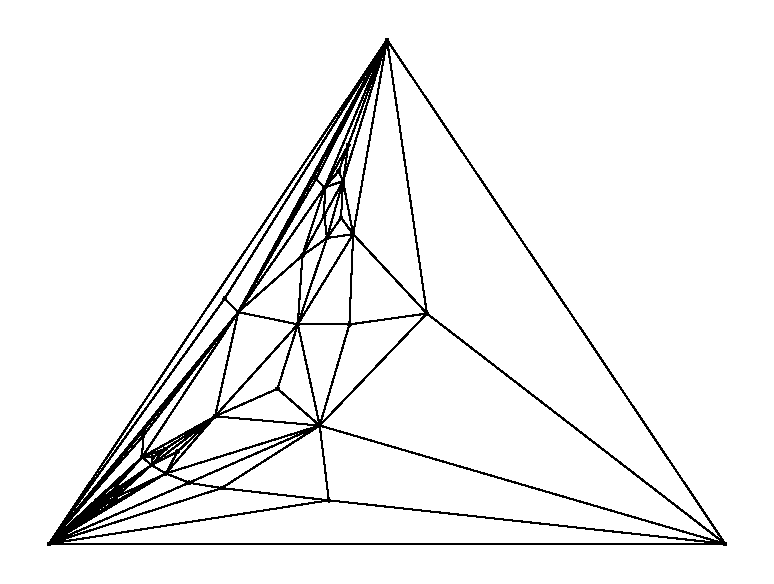
\includegraphics[width = \textwidth]{../output/Q9-random-4013.pdf}
          \caption{Graph number 4}
      \end{subfigure}
      \hfill
      \caption{Four of the randomly generated maximal planar graphs.}
      \label{randomplots}
  \end{figure}

\textbf{Question 10}\quad 
Suppose we want to check if a graph \(G\) with \(n\) edges is planar. Then it
contains at most \(O(n)\) vertices. To find the core of \(G\), we iterate over
all the vertices and remove the ones of degree \(\leq 3\). Since computing the
degree of any vertex (i.e.\ the length of the list containing its neighbourhood)
takes constant time, finding the core has complexity \(O(n)\). In the worst
case, \(G\) is its own core. Now we simply start with a vertex and extend the
path one step at a time till it closes into a cycle \(C\) with a chord, this
taking another \(O(n)\) steps. To find the component of a particular vertex in
\(G-C\), we pick a vertex and keep adding neighbours of vertices found so far.
This takes \(O(n^2)\) steps, and we do this for \(O(n)\) vertices in the worst
case hence finding the bridges has complexity \(O(n^3)\). 

In the worst case, the cycle we find has length \(O(n)\) and there are \(O(n)\)
components. Then checking if each pair of components interleaves takes
\(O(n)\) steps (traversing once through the cycle, keeping track of possible
interleaves seen so far), hence the interleaf graph takes \(O(n^3)\) steps to construct and has size \(O(n)\). Checking if the interleave graph is bipartite then has complexity \(O(n^2)\).

Hence a single iteration of the algorithm has complexity \(O(n^3)\). Each
iteration, we remove (in the worst case) one edge from \(G\) hence the entire
algorithm takes \(O(n^4)\) steps to check for planarity.

\subsubsection*{Appendix A. \quad Random maximal planar graphs}
We present the output produced after running the algorithm to
randomly generate maximal planar graphs on \(40\) vertices (labelled
\(\texttt{0}\) to \(\texttt{39}\)). One evidence that the algorithm works
properly is to observe that each graph has \(114 = 3\times 40 - 6\) edges,
arranged in a \(6\times 19\) grid. Each grid should be read row-by-row, left to
right and top to bottom. Across twenty such graphs, the mean number of edges
added before the first violation of planarity is 42.55.
\verbatimfont{\footnotesize\ttfamily}
\begin{enumerate}[1.]
    \item \verbatiminput{../output/Q9-maximal-5.txt} 
    \item \verbatiminput{../output/Q9-maximal-9.txt} 
    \item \verbatiminput{../output/Q9-maximal-12.txt} 
    \item \verbatiminput{../output/Q9-maximal-13.txt} 
\end{enumerate}

\subsubsection*{Appendix B: Programs}

\underline{\texttt{graphs.py}}
\lstinputlisting{../src/graphs.py}

\underline{\texttt{bridges.py}}
\lstinputlisting{../src/bridges.py}

\underline{\texttt{core.py}}
\lstinputlisting{../src/core.py}

\underline{\texttt{main.py}}
\lstinputlisting{../src/main.py}

\end{document}
